%!TEX root = ../Thesis.tex

\section{Recurent Neural Network}

The Skip-gram model can be interpreted as a Feedforward Neural Network (FFNN). This class of neural networks have the shortcoming that the require a fixed input size, thus they can only look a fixed amount of steps back and forward in history. This can be a problem when analyzing sentences, because the amount of words in a sentence isn't fixed and there isn't a well defined window size for the surrounding words.

The Recurrent Neural Networks (RNN) overcome this shortcoming by having an internal state. In principal this allows the network to take a sequence of vectors and consider the entire history. The sequence can be of any size, but each vector must be of the same size. In the case of sentences a fixed vector size is not an issue when considering a fixed vocabulary.

In practice it turns out that the RNN forgets the past and only have a short memory. Another model called Long-Short-Term-Memory (LSTM) extends the RNN and have been shown to have better performance \cite{alexgraves}. The ideas are however still the same, thus to understand the LSTM model a basic understanding of the RNN model is valuable.

\subsection{Forward pass}

\begin{figure}[h]
	\centering
	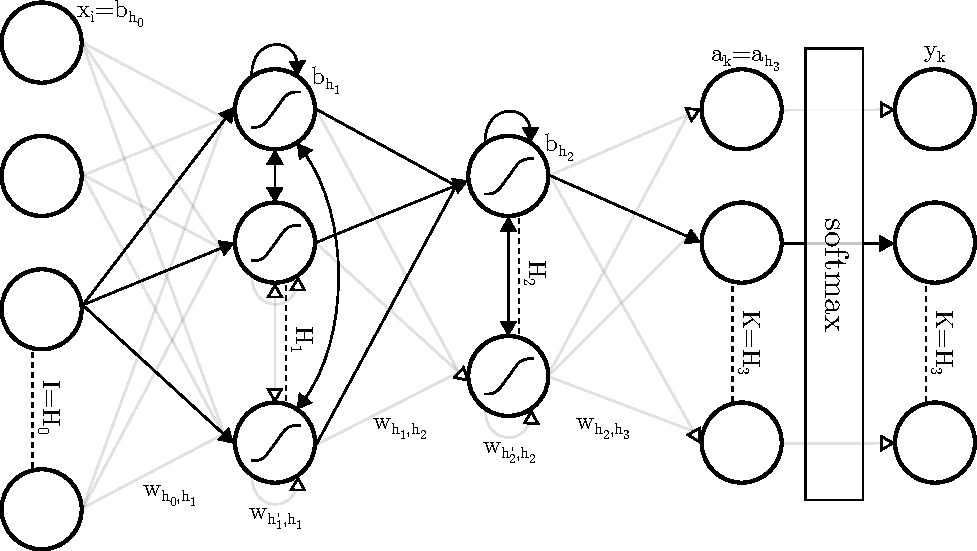
\includegraphics[scale=0.7]{theory/rnn-network}
	\caption{Visualization of a single iteration in a Recurent Neural Network.}
	\label{fig:theory:rnn:rnn-network}
\end{figure}

Consider Figure \ref{fig:theory:rnn:rnn-network} but without the extra internal connections, such that it is just a feedforward neural network. The elements in the input vector is then denoted $x_{i}, i \in [1, I]$, the corresponding input for the hidden layer is $a_{h_\ell}, h_\ell \in [1, H_\ell]$ with an activation $b_{h_\ell}, _\ell \in [1, H_\ell]$. Finally there is the network output $a_{k}, k \in [1, K]$. This is just like the notation used for the FFNN.

However since a sequence of $\mathbf{x}$ vectors will be used later, a $t \in [1, T]$ is added to the notation. Note that just because a $t$ symbol is used, the RNN model generalizes to non-time dependent datasets as well. In the case of semantic text analysis the sequence $\{\mathbf{x}^t\}_{t=1}^T$ will refer to a sequence of words represented using 1-of-V encoding. The total sequence then contains a complete sentences or paragraph. 

Now recall that in a FFNN the input for the hidden layer is:
\begin{equation}
a_{h_\ell}^t = \sum_{h_{\ell-1}=1}^{H_{\ell-1}} w_{h_{\ell-1}, h_\ell} b_{h_{\ell-1}}^t \quad \forall \ell \in [1, L+1]
\end{equation}

In the case of a RNN the input for the hidden layer ($a_{h_\ell}^t$) is expanded, such that i depends on the hidden activation for the previous time iteration ($b_{h_\ell}^{t-1}$):
\begin{equation}
a_{h_\ell}^t = \sum_{h_{\ell-1}=1}^{H_{\ell-1}} w_{h_{\ell-1}, h_\ell} b_{h_{\ell-1}}^t + \sum_{h'_\ell=1}^{H_\ell} w_{h'_\ell h_\ell} b_{h'_\ell}^{t-1} \quad \forall \ell \in [1, L]
\end{equation}

Just as with the FFNN $\theta$ is the activation function:
\begin{equation}
b_{h_\ell}^t = \theta(a_{h_\ell}^t) \quad \forall \ell \in [1, L]
\end{equation}

In order to fully calculate the forward pass, $b_{h'_\ell}^0$ needs to be initialized to some value. Usually it is set to $0$ however there are other choices.

\subsection{Backward pass}

Just like \textit{error backpropagation} is used to calculate the loss function derivatives with respect to the weights in a FFNN, similar method exists for the RNN. The method is called \textit{backpropagation through time} (BPTT). Is almost identical to backpropagation in the feedforward network, except that it doesn't just go backward though the layers but also goes backward though time ($t$), or in this case the sequence of words. \cite{alexgraves}

Consider again the log-likelihood function for a multiclass problem, where the probabilities $y_k^t$ are calculated using a softmax. However this time the probability must be considered for all time steps.
\begin{align}
\mathcal{L} &= - \sum_{t=1}^T \sum_{k=1}^K t_k^t \ln(y_k^t) \\
y_k^t &= \frac{\mathrm{exp}(a_k^t)} {\sum_{k'=1}^K \mathrm{exp}(a_{k'}^t)}
\end{align}

Just like in the FFNN the derivatives with respect to the first weights are considered as a starting point. However because of the time dependency the chain rule results in a sum over the time steps:
\begin{equation}
\frac{\partial \mathcal{L}}{\partial w_{h_0, h_1}} = \sum_{t=1}^T \frac{\partial \mathcal{L}}{\partial a_{h_1}^t} \frac{\partial a_{h_1}^t}{w_{h_0, h_1}}
\label{eq:theory:rnn:startingpoint}
\end{equation}

Now the $\delta$ definition is introduced:
\begin{equation}
\delta_{h_\ell}^t \defeq \frac{\partial \mathcal{L}}{\partial a_{h_\ell}^t}
\end{equation}

Applying this definition and using $ \frac{\partial a_{h_1}^t}{w_{h_0, h_1}} = x_{h_0}^t$,  \eqref{eq:theory:rnn:startingpoint} becomes:
\begin{equation}
\frac{\partial \mathcal{L}}{\partial w_{h_0, h_1}} = \sum_{t=1}^T \delta_{h_1}^t x_{h_0}^t = \sum_{t=1}^T \delta_{h_1}^t b_{h_0}^t 
\end{equation}

The next step is now to derive the equation for $\delta_{h_1}^t$, this is a bit tricky because both $a_{h_2}^t$ and $a_{h_1}^{t+1}$ is affected by $a_{h_1}^t$, thus the chain rule gives two sums:
\begin{equation}
\delta_{h_1}^t = \frac{\partial \mathcal{L}}{\partial a_{h_1}^t}
= \sum_{h_2 = 1}^{H_2} \frac{\partial \mathcal{L}}{\partial a_{h_2}^t} \frac{\partial a_{h_2}^t}{\partial a_{h_1}^t}
+ \sum_{h'_1 = 1}^{H_1} \frac{\partial \mathcal{L}}{\partial a_{h'_1}^{t+1}} \frac{\partial a_{h'_1}^{t+1}}{\partial a_{h_1}^t}
\end{equation}

Again the chain rule is used, this time to get $\frac{\partial b_{h_1}^t}{\partial a_{h_1}^t}$:
\begin{equation}
\begin{aligned}
\delta_{h_1}^t = \frac{\partial \mathcal{L}}{\partial a_{h_1}^t}
&= \sum_{h_2 = 1}^{H_2} \frac{\partial \mathcal{L}}{\partial a_{h_2}^t} \frac{\partial a_{h_2}^t}{\partial b_{h_1}^t} \frac{\partial b_{h_1}^t}{\partial a_{h_1}^t}
+ \sum_{h'_1 = 1}^{H_1} \frac{\partial \mathcal{L}}{\partial a_{h'_1}^{t+1}} \frac{\partial a_{h'_1}^{t+1}}{\partial b_{h_1}^t} \frac{\partial b_{h_1}^t}{\partial a_{h_1}^t} \\
&= \frac{\partial b_{h_1}^t}{\partial a_{h_1}^t} \left(\sum_{h_2 = 1}^{H_2} \frac{\partial \mathcal{L}}{\partial a_{h_2}^t} \frac{\partial a_{h_2}^t}{\partial b_{h_1}^t}
+ \sum_{h'_1 = 1}^{H_1} \frac{\partial \mathcal{L}}{\partial a_{h'_1}^{t+1}} \frac{\partial a_{h'_1}^{t+1}}{\partial b_{h_1}^t} \right) \\
&= \theta'(a_{h_1}^t) \left( \sum_{h_2=1}^{H_2} \delta_{h_2}^t w_{h_1, h_2}
+ \sum_{h'_1=1}^{H_1} \delta_{h_1}^{t+1} w_{h'_1, h_1} \right)
\label{eq:theory:rnn:bprop-delta1}
\end{aligned}
\end{equation}

Note that $\delta_{h_1}^{t}$ is not yet completely well defined, because for $t = T$ there is an unknown $\delta_{h_1}^{T+1}$ term. This is set to zero ``since no error is received from beyond the end of the sequence'' \cite{alexgraves}.

From \eqref{eq:theory:rnn:bprop-delta1} its seen that the next step is to derive $\delta_{h_2}^t$. This was also the case with the FFNN and it what shown that $\delta_{h_2}$ was not much different from $\delta_{h_1}^{t}$ and generalizing it was the natural choice. The same is the case for the RNN. Generalizing then gives:
\begin{equation}
\begin{aligned}
\delta_{h_\ell}^t = \theta'(a_{h_\ell}^t) \left( \sum_{h_{\ell+1}=1}^{H_{\ell+1}} \delta_{h_{\ell +1}}^t w_{h_\ell, h_{\ell + 1}}
+ \sum_{h'_\ell=1}^{H_\ell} \delta_{h_\ell}^{t+1} w_{h'_\ell, h_\ell} \right), && \forall \ell \in [1, L]
\end{aligned}
\end{equation}

Because $h_{L+2}$ isn't defined, it is seen from the generalization that $\delta_{L+1}^t$ is again a special case:
\begin{equation}
\delta_{L+1}^t = \delta_{k}^t = \frac{\partial \mathcal{L}}{\partial a_{h_k}^t} = \sum_{k'=1}^K \frac{\partial \mathcal{L}}{\partial y_{k'}^t} \frac{\partial y_{k'}^t}{\partial a_k^t}
\end{equation}

This is similar to the FFNN case with the exception that there is a time step, thus the same equation is obtained:
\begin{equation}
\delta_{k}^t = y_k^t - t_k^t
\end{equation}

This set of equation allows calculation of all $\delta_{h_\ell}^t$, however the derivatives with respect to the other weight still need to be considered.
\begin{equation}
\frac{\partial \mathcal{L}}{\partial w_{h'_1, h_1}} = \sum_{t=1}^T \frac{\partial \mathcal{L}}{\partial a_{h_1}^t} \frac{\partial a_{h_1}^t}{\partial w_{h'_1, h_1}} = \sum_{t=1}^T \delta_{h_1}^t b_{h'_1}^{t-1}
\end{equation}

Generalizing this both for the weights between layer $w_{h_{\ell - 1}, h_\ell}$ and between time steps $w_{h'_{\ell}, h_\ell}$, one gets:
\begin{align}
\frac{\partial \mathcal{L}}{\partial w_{h'_\ell, h_\ell}} &= \sum_{t=1}^T \frac{\partial \mathcal{L}}{\partial a_{h_\ell}^t} \frac{\partial a_{h_\ell}^t}{\partial w_{h'_\ell, h_\ell}} = \sum_{t=1}^T \delta_{h_\ell}^t b_{h'_\ell}^{t-1}, && \forall \ell \in [1, L] \\
\frac{\partial \mathcal{L}}{\partial w_{h_{\ell - 1}, h_\ell}} &= \sum_{t=1}^T \frac{\partial \mathcal{L}}{\partial a_{h_\ell}^t} \frac{\partial a_{h_\ell}^t}{\partial w_{h_{\ell-1}, h_\ell}} = \sum_{t=1}^T \delta_{h_\ell}^t b_{h_{\ell-1}}^t, && \forall \ell \in [1, L + 1] 
\end{align}
